SmallWorld Lord of Ring est un jeu de plateau 2 Joueurs pour toute la famille. Rejoignez le monde du seigneur des anneaux tout en jouant au célèbre SmallWord.
\newline
\begin{center}
Serez-vous le plus fort à collecter tous les anneaux de pouvoir ?
\end{center}
\begin{center}
Ainsi vous pourrez récupérer l'anneau unique pour dominer le monde !
\end{center}

\subsection{Généralités}

Morgoth, un seigneur du mal très puissant, terrorisait la terre du milieu. Un alliance d'un nouveau genre fut forgée entre les elfes, les orques, et les nains pour tenter de l'arrêter. Après une bataille féroce, Morgoth fut défait devant la montagne du destin.
\newline
\newline
Afin d'empêcher une nouvelle guerre, les peuples choisirent d'équilibrer les forces sur la terre du milieu. Ainsi, avec l'aide bienveillante de Sauron, ils créent un certain nombre d'anneaux de pouvoir, qu'ils distribuent à parts égales aux elfes, orques et nains.
\newline
 Les hommes, ayant collaboré avec Morgoth alors qu'ils étaient dans la coalition contre lui, ont été punis, et n'ont pas eu d'anneau. Les Hobbits n'ont eux pas eu d'anneaux car ils s'occupaient trop de leurs maisons pendant la grande guerre.
\newline
\newline
Ainsi, les grands peuples ne se querelleront plus car ils détiennent tous des pouvoirs équivalents.
\newline
\newline
Mais ce que les anciens ne savaient pas, c'est que le contrôle de la majorité des anneaux de pouvoir peut bouleverser la vie sur la terre du milieu. En effet, le fourbe Sarumane, sorcier humain et chef du conseil blanc, a dans le secret créé un enchantement magique. Au bout d'un temps imparti, le contrôle de la majorité des anneaux de contrôle vous permettra de retrouver l'anneau unique, capable de contrôler tous les autres anneaux, pour conquérir le monde.
\newline
\newline
Chaque combat peut changer l'équilibre des forces. Les anneaux ont été forgés de manière à ce que si le possesseur initial mourrait, l'anneau serait détruit pour empêcher le cumul d'anneau. Les elfes n'ont pas inventé l'art de la guerre, ainsi ils peuvent aléatoirement fuire avant de perdre un combat. 
\newline
Pour tous les autres, la bravoure domine : la perte d'un combat implique la mort du perdant. Cependant, tous les combats n'ont pas tous un gagnant. En revanche, l'abulcasis n'ayant pas été inventé, et Gandalf étant en vacances à Isengard, il n'est pas possible de soigner les unités.
\newline
\newline
Les anneaux de contrôle sont récessifs entre eux. Ainsi, quand 2 unités du même peuple se rencontrent, un seul anneau garde son pouvoir. Ainsi, si 10 unités se retrouvent pour festoyer, seulement 1 anneau de contrôle sera actif. Les orques ont cependant réussi à contourner une partie de cet effet.
\newpage
Ce secret est arrivé jusqu'à vous, chef de votre peuple, et vous convoitez l'anneau unique. L'ère de paix a prix fin suite aux attaques d'orques sur les fermes des hommes.  Vous savez qu'il ne vous reste plus beaucoup de temps, et que d'autres chefs qui ont la même information pourraient tenter de lever une armée pour devenir le maître du monde.
\newline
\begin{center}
Serez-vous le plus fort à collecter tous les anneaux de pouvoir ?
\end{center}
\begin{center}
Ainsi vous pourrez récupérer l'anneau unique pour dominer le monde !
\end{center}

\subsection{Prise en main rapide}

Il vous est possible de créer une nouvelle partie, ou de charger une ancienne.
Il existe 3 types de parties différentes
\begin{itemize}
\item Partie Comté : partie démo, peu de tours et d'unités
\item Partie Erebor : partie moyenne
\item Partie Terre du milieu : grande partie, grand nombre de tours et d'unités
\newline
\end{itemize}
Après avoir rentré un nom de joueur et choisi un type (au choix entre elfe, orque, nain), vous
pouvez commencer la partie. Toutes vos unités sont concentrées en 1 point de la carte.
\newline
\newline
A chaque début de tour, le nombre d'anneau par joueur est décompté. Le nombre de déplacement possible est initialisé à 1 par unité. 
Vous pouvez vous déplacer sur une case qui coûte moins ou le exactement le coût de cette case. Les coûts des cases varient en fonction des unités et du terrain des cases. 
\newline
\newline
Vous pouvez aussi attaquer une unité ennemie. Le combat se fera de manière aléatoire, l'attaque sera pondérée par les points de vie restants de l'unité. Vous pouvez soit gagner, soit perdre, soit faire match nul au combat. Les points de vie ne peuvent pas se soigner.
Toutes les unités ont 2 d'attaque et 1 de défense.
\newline
\newline
Le gagnant de l'anneau unique est celui qui totalise le plus d'anneau à la fin du dernier tour de jeu.

\newpage
\subsection{Type de partie}

Il y a 3 types de parties. Ces trois types se basent sur les mêmes règles générales, et ne font varier que des spécificités de ces parties. En voici la description.
\subsubsection{Partie Comté}
C'est le mode de jeu Démo, il n'y a que 5 tours. Le terrain est composé de 6*6 cases, et il n'y a seulement que 4 unités par joueur. C'est le mode idéal pour apprendre les commandes du jeu.
\subsubsection{Partie Erebor}
C'est le mode de jeu intermédiaire. Il y a 20 tours. Le terrain est composé de 10*10 cases, et il y a 6 unités par joueur.
\subsubsection{Partie Terre du milieu}
C'est le mode de jeu normal. Il y a 30 tours. Le terrain est composé de 14*14 cases, et il y a 8 unités par joueur. C'est le format de partie conseillé.

\subsection{Règles selon les Type d'unités}
\subsubsection{Règles générales}
Les déplacements et les attaques coûtent globalement tous 1, mais des exceptions seront présentés dans les sections suivantes.
\newline
\newline
La partie est trop rapide dans le temps pour que de nouvelles unités rejoignent le champ de bataille. Ainsi, aucune unité ne peut-être créée.
\newline
 De plus, les orques ont rattrapé leur retard sur les nains et les elfes dans les techniques de combat : ils sont maintenant capables de toucher et de tuer leurs ennemis pendant un combat.
\newline
\newline
Toutes les unités ont une attaque de 2 et une défense de 1.
\newline
Les elfes n'ont pas de stocks de flèches illimités, il ne peuvent pas non plus tuer à plus de 100 mètres de leur cible. Toutes les unités doivent être sur la case de l'unité adverse pour attaquer.
\newline
Les anneaux de contrôle sont normalement récessifs entre eux. Ainsi, quand 2 unités du même peuple se rencontrent, un seul anneau garde son pouvoir. Il en est autrement pour les orques.
\newline
\newline
Si les règles du jeu ne sont pas respectées, les erreurs sont affichées en bas à gauche dans un cadre noir. Un exemple d'erreur est présenté en Figure 11.

\newpage
\subsubsection{Elfe}
Le peuple elfe a depuis des générations vécu dans les forêts de Mirkwood, c'est pourquoi il peut se déplacer 2 fois plus rapidement sur ces cases.
\newline
 En revanche, les elfes ne peuvent pas traverser le désert parce qu'ils ne trouvent pas l'eau nécessaire à leur confort capillaire.
\newline
\newline
Les elfes maîtrisent au mieux l'art de la guerre. Ainsi, quand le combat est perdu, il leur est donnée la possibilité aléatoirement de fuir sur une case adjacente, mais avec plus qu'1 point de vie.
\newline
  S'il n'y a pas de possibilité, l'unité meurt.

\begin{figure}[!h]
\centering
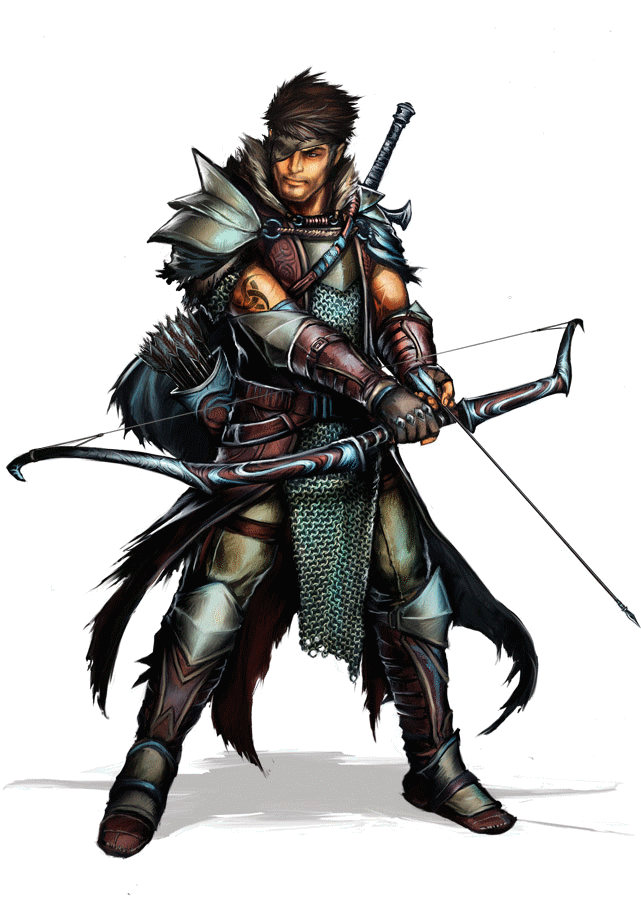
\includegraphics[scale=0.10]{img/elf.png}
\caption{Un elfe}
\end{figure}

\subsubsection{Orque}

Le peuple orque a retrouvé les descendants des forgerons des anneaux, et en les torturant des mois durant, les orques ont réussi à créer un sort qui récupère l'anneau sur le corps mort de l'ennemi à la fin du combat ! Ainsi, les orques peuvent cumuler les anneaux.
\newline
\newline
Les anneaux de contrôle sont normalement récessifs entre eux. Ainsi, quand 2 unités du même peuple se rencontrent, un seul anneau garde son pouvoir. Cependant, les orques ont réussi seulement à garder l'effet des anneaux volés lors des combats.
\newline
\newline
Le peuple orque est à l'aise dans la plaine, il peut se rassasier de toutes les denrées qu'il ne trouve pas au Mordor. C'est pourquoi il s'y déplace 2 fois plus vite. 
\newline Cependant, le sort des anneaux ne fonctionne pas sur les cases Forêt, ainsi, les anneaux des orques n'ont plus d'effet en présence de ce terrain.

\begin{figure}[!h]
\centering
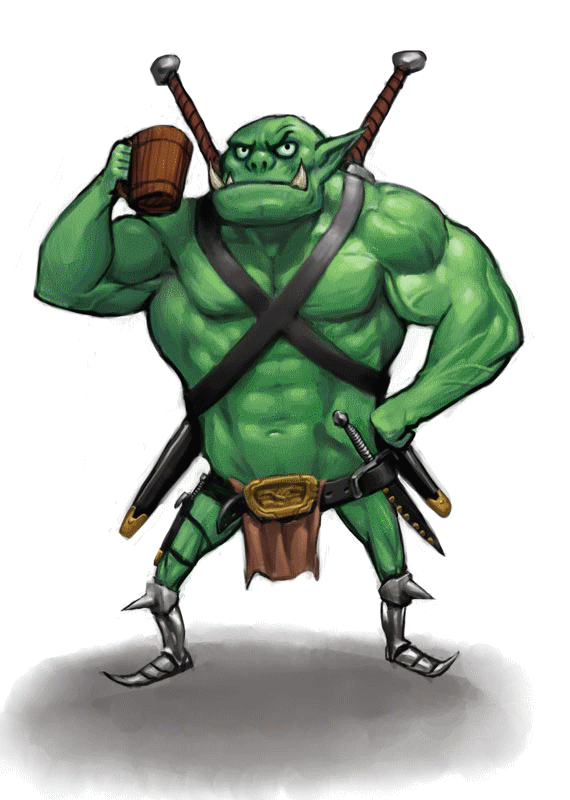
\includegraphics[scale=0.10]{img/orc.png}
\caption{Un orc}
\end{figure}

\subsubsection{Nain}
Le peuple nain a des capacités spéciales quand il se trouve sur les plaines. Il est capable de fabriquer avec du blé et de l'avoine des potages aphrodisiaques qui leur permettront de se déplacer 2 fois plus vite, mais qui leur empêchera d'utiliser leurs anneaux.
\newline
 Ainsi, les anneaux des nains ne seront pas comptabilisés sur les cases Plaine.
\newline
\newline
Le peuple nain a été élevé dans les montagnes, quelles soient bleues, ou qu'elles soient d'Erebor. Les nains sont capables de se déplacer très vite dans les montagnes, plus rapidement même que les autres types de créature, mais pas aussi vite que les aigles de Galadriel.
\newline Ainsi, leur déplacement ne coûtera rien sur les cases Montagne.

\begin{figure}[ht!]
\centering
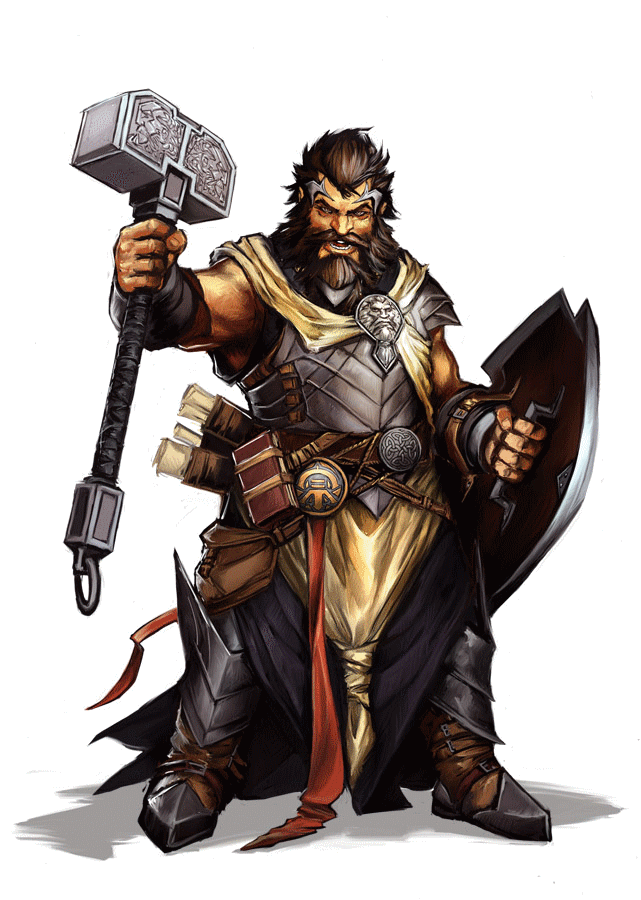
\includegraphics[scale=0.10]{img/dwarf.png}
\caption{Un nain}
\end{figure}

\subsection{Types de terrains}
Il existe 4 types de terrains représentés comme suit :

\begin{figure}[ht]
\begin{minipage}[b]{0.45\linewidth}
\centering
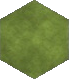
\includegraphics[scale=1]{img/plaine.png}
\caption{Une case plaine}
\label{fig:figure1}
\end{minipage}
\hspace{0.5cm}
\begin{minipage}[b]{0.45\linewidth}
\centering
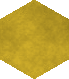
\includegraphics[scale=1]{img/desert.png}
\caption{Une case desert}
\label{fig:figure2}
\end{minipage}
\end{figure}

\begin{figure}[ht]
\begin{minipage}[b]{0.45\linewidth}
\centering
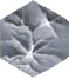
\includegraphics[scale=1.35]{img/montagne.png}
\caption{Une case montagne}
\label{fig:figure1}
\end{minipage}
\hspace{0.5cm}
\begin{minipage}[b]{0.45\linewidth}
\centering
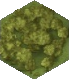
\includegraphics[scale=1]{img/foret.png}
\caption{Une case forêt}
\label{fig:figure2}
\end{minipage}
\end{figure}